\chapterWithSubtitle{Dynamic Programming}{March 11, 2021}

\section{Recursion Types}

\begin{itemize}
    \item Divide and Conquer
    \item Backtracking
    \item \textbf{Dynamic Programming}:
    \begin{itemize}
        \item Smart recursion with memoization
    \end{itemize}
\end{itemize}

\section{Dynamic Programming}

\subsection{Fibonacci Sequence}
\begin{itemize}
    \item The Fibonacci sequence is defined as $F(n) = F(n - 1) + F(n - 2)$.
    \item The running time is $T(n)$, defined by the number of additions in $F(n)$.
    \item[] 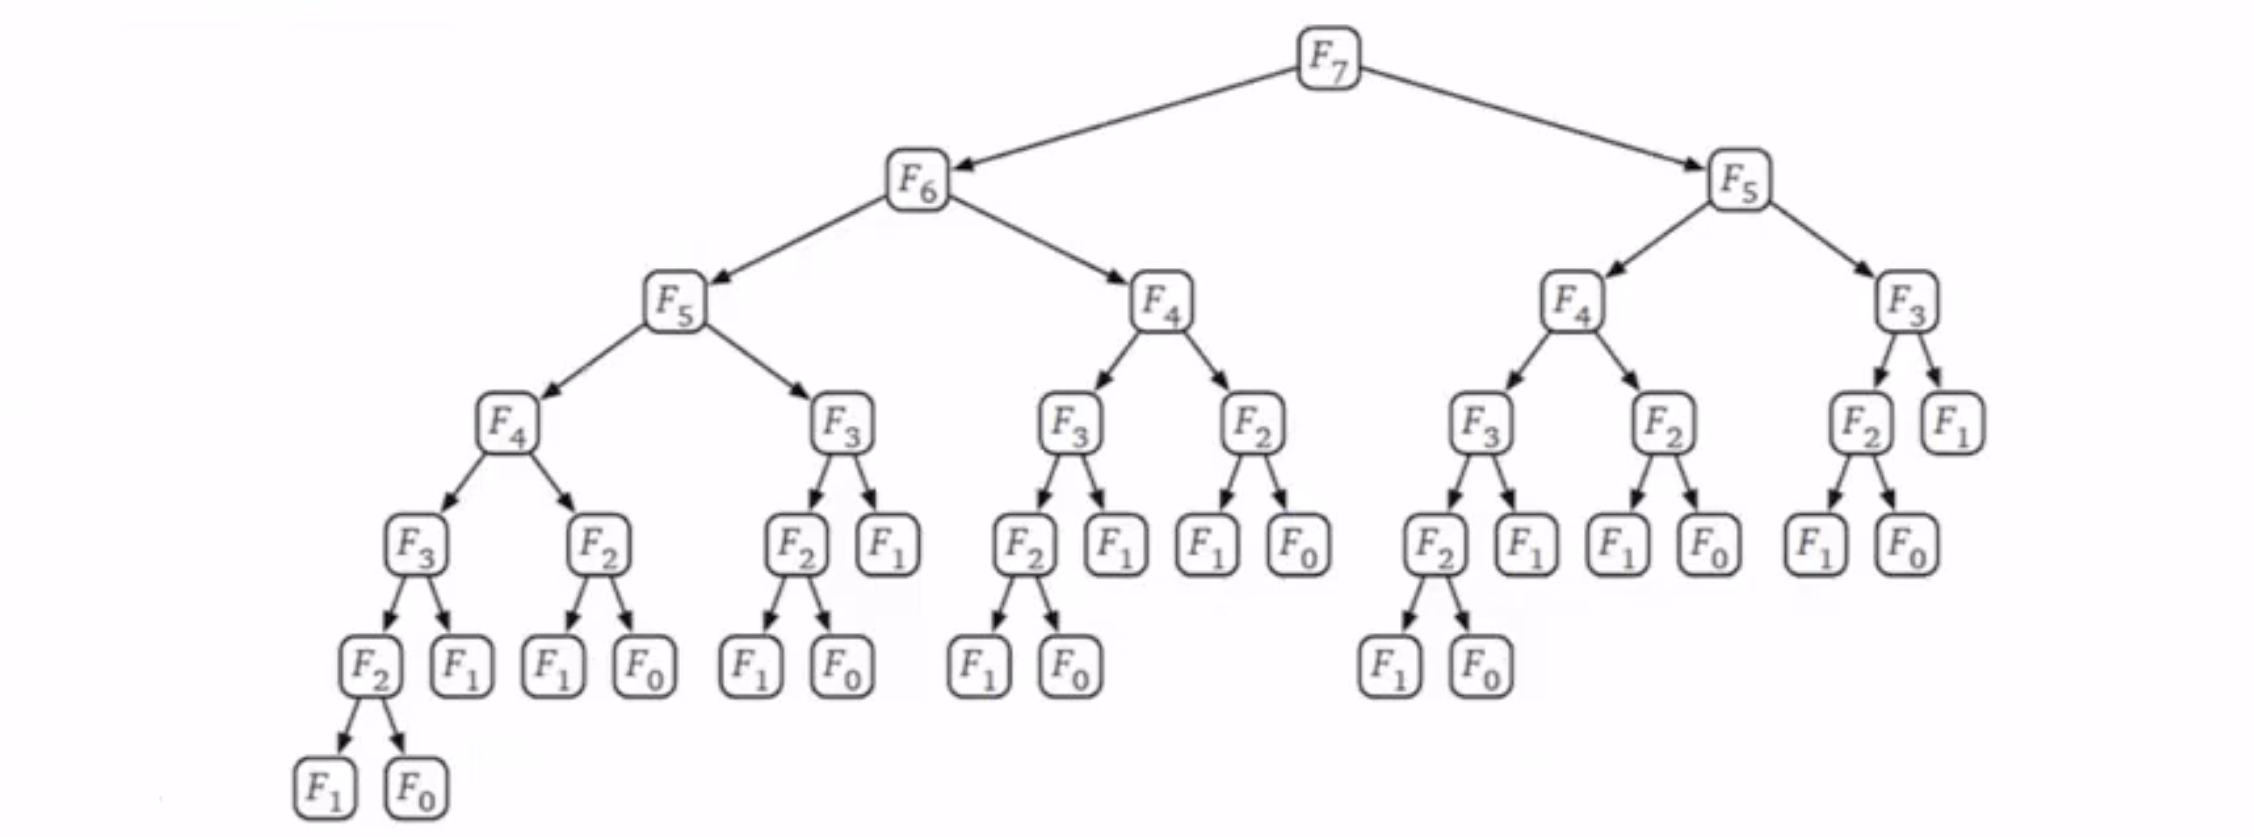
\includegraphics[width=\textwidth]{lecture13/images/fib-without-memo.png}
    \item $T(n) = T(n - 1) + T(n - 2) + 1$, $T(n) = O(c^n)$ for some $c$, so it is exponential in $n$.
    \item The recursive algorithm is slow because it computes the same Fibonacci numbers multiple times.
    \item To make this faster, we can use \textit{Memoization}, where we write down the results of recursive calls and look them up later.
    \item An array $F[n]$ where $F[i]$ stores the result of $F(i)$.
    \item We evaluate from bottom up: $i = 2, 3...$.
    \item[] 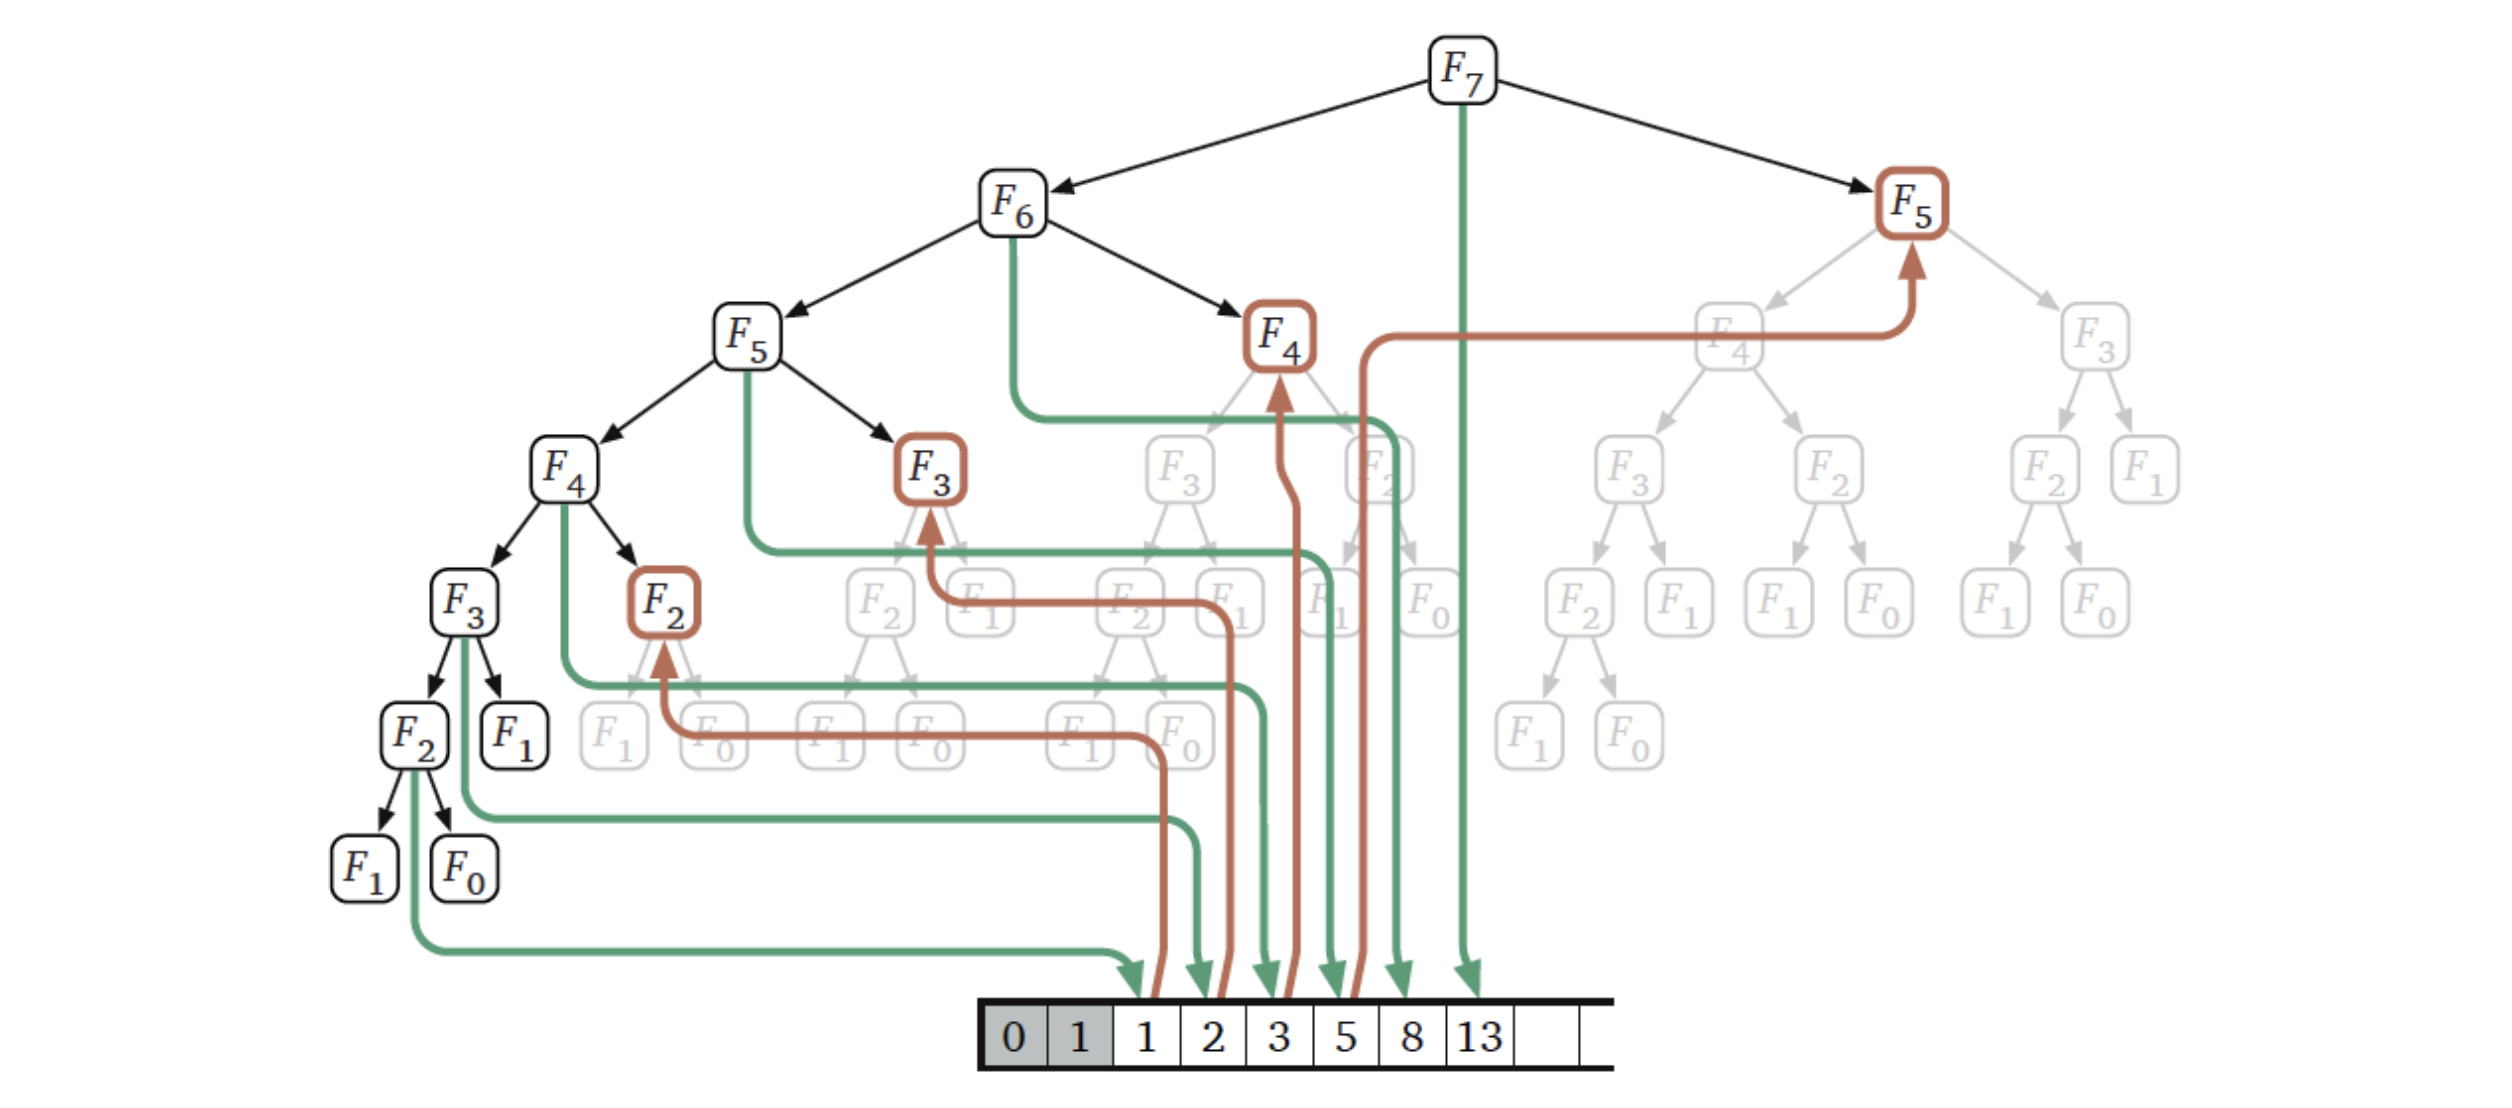
\includegraphics[width=\textwidth]{lecture13/images/fib-with-memo.png}
    \item Dynamic programming is essentially finding a recursion that can be effectively/efficiently memoized. This leads to a polynomial time algorithm if the number of distinct sub-problems is polynomial in input size.
    \item In this example, we do not really need an entire array; we can just save only the previous two numbers and add them to get the next number.
\end{itemize}

\subsection{Dynamic Programming Rules}
\begin{itemize}
    \item Dynamic programming is not about filling tables. It is about finding a smart recursion. First, find a correct recursion.
    \item Use memoization to avoid recomputation of common solutions, hence optimizing running time and space.
    \begin{itemize}
        \item Allocate a data structure (typically an array or multi-dimensional array that can hold values for each of the sub-problems).
        \item Order the computation of the sub-problems starting from the base case. This will usually be an iterative solution from the bottom up.
    \end{itemize}
\end{itemize}

\subsection{Designing Dynamic Programming}
\begin{itemize}
    \item Find a "smart" recursion
    \begin{itemize}
        \item Formulate the sub-problem
        \item The number of distinct sub-problems is small, and polynomial in the original problem size.
    \end{itemize}
    \item Memoization
    \begin{itemize}
        \item Identify distinct sub-problems
        \item Choose a memoization data structure
        \item Identify dependencies and find a good evaluation order
        \item Find an iterative algorithm replacing recursive calls with array lookups
    \end{itemize}
\end{itemize}

\subsection{Longest Increasing Subsequence}
\begin{itemize}
    \item[] \lstinputlisting{lecture13/code/longest-increasing-subsequence.sudo}
    \item Memorizing \texttt{LIS\_smaller($A[1...n]$, infinity)} generates $O(n^2)$ sub-problems.
    \item The running time after memorizing recursion is $O(n^2)$ because it is $O(1)$ to assemble the answer from two memoized recursive calls.
    \item $O(n^2)$ space is required for memoization.
    \item \texttt{LIS($i$, $j$)} is the length of the longest increasing subsequence in $A[1...i]$ among numbers less than $A[j]$ (define $i < j$).
    \begin{itemize}
        \item \textit{Base Case}: $\texttt{LIS($0$, $j$)} = 0$ for $1 \leq j \leq n + 1$.
        \item \textit{Recursive Relation}:
        \begin{itemize}
            \item $\texttt{LIS($i$, $j$)} = \texttt{LIS($i - 1$, $j$)}$ for $A[i] > A[j]$
            \item $\texttt{LIS($i$, $j$)} = \max(\texttt{LIS($i - 1$, $j$)}, 1 + \texttt{LIS($i - 1$, $i$)})$ for $A[i] \leq A[j]$
        \end{itemize}
    \end{itemize}
    \item[] 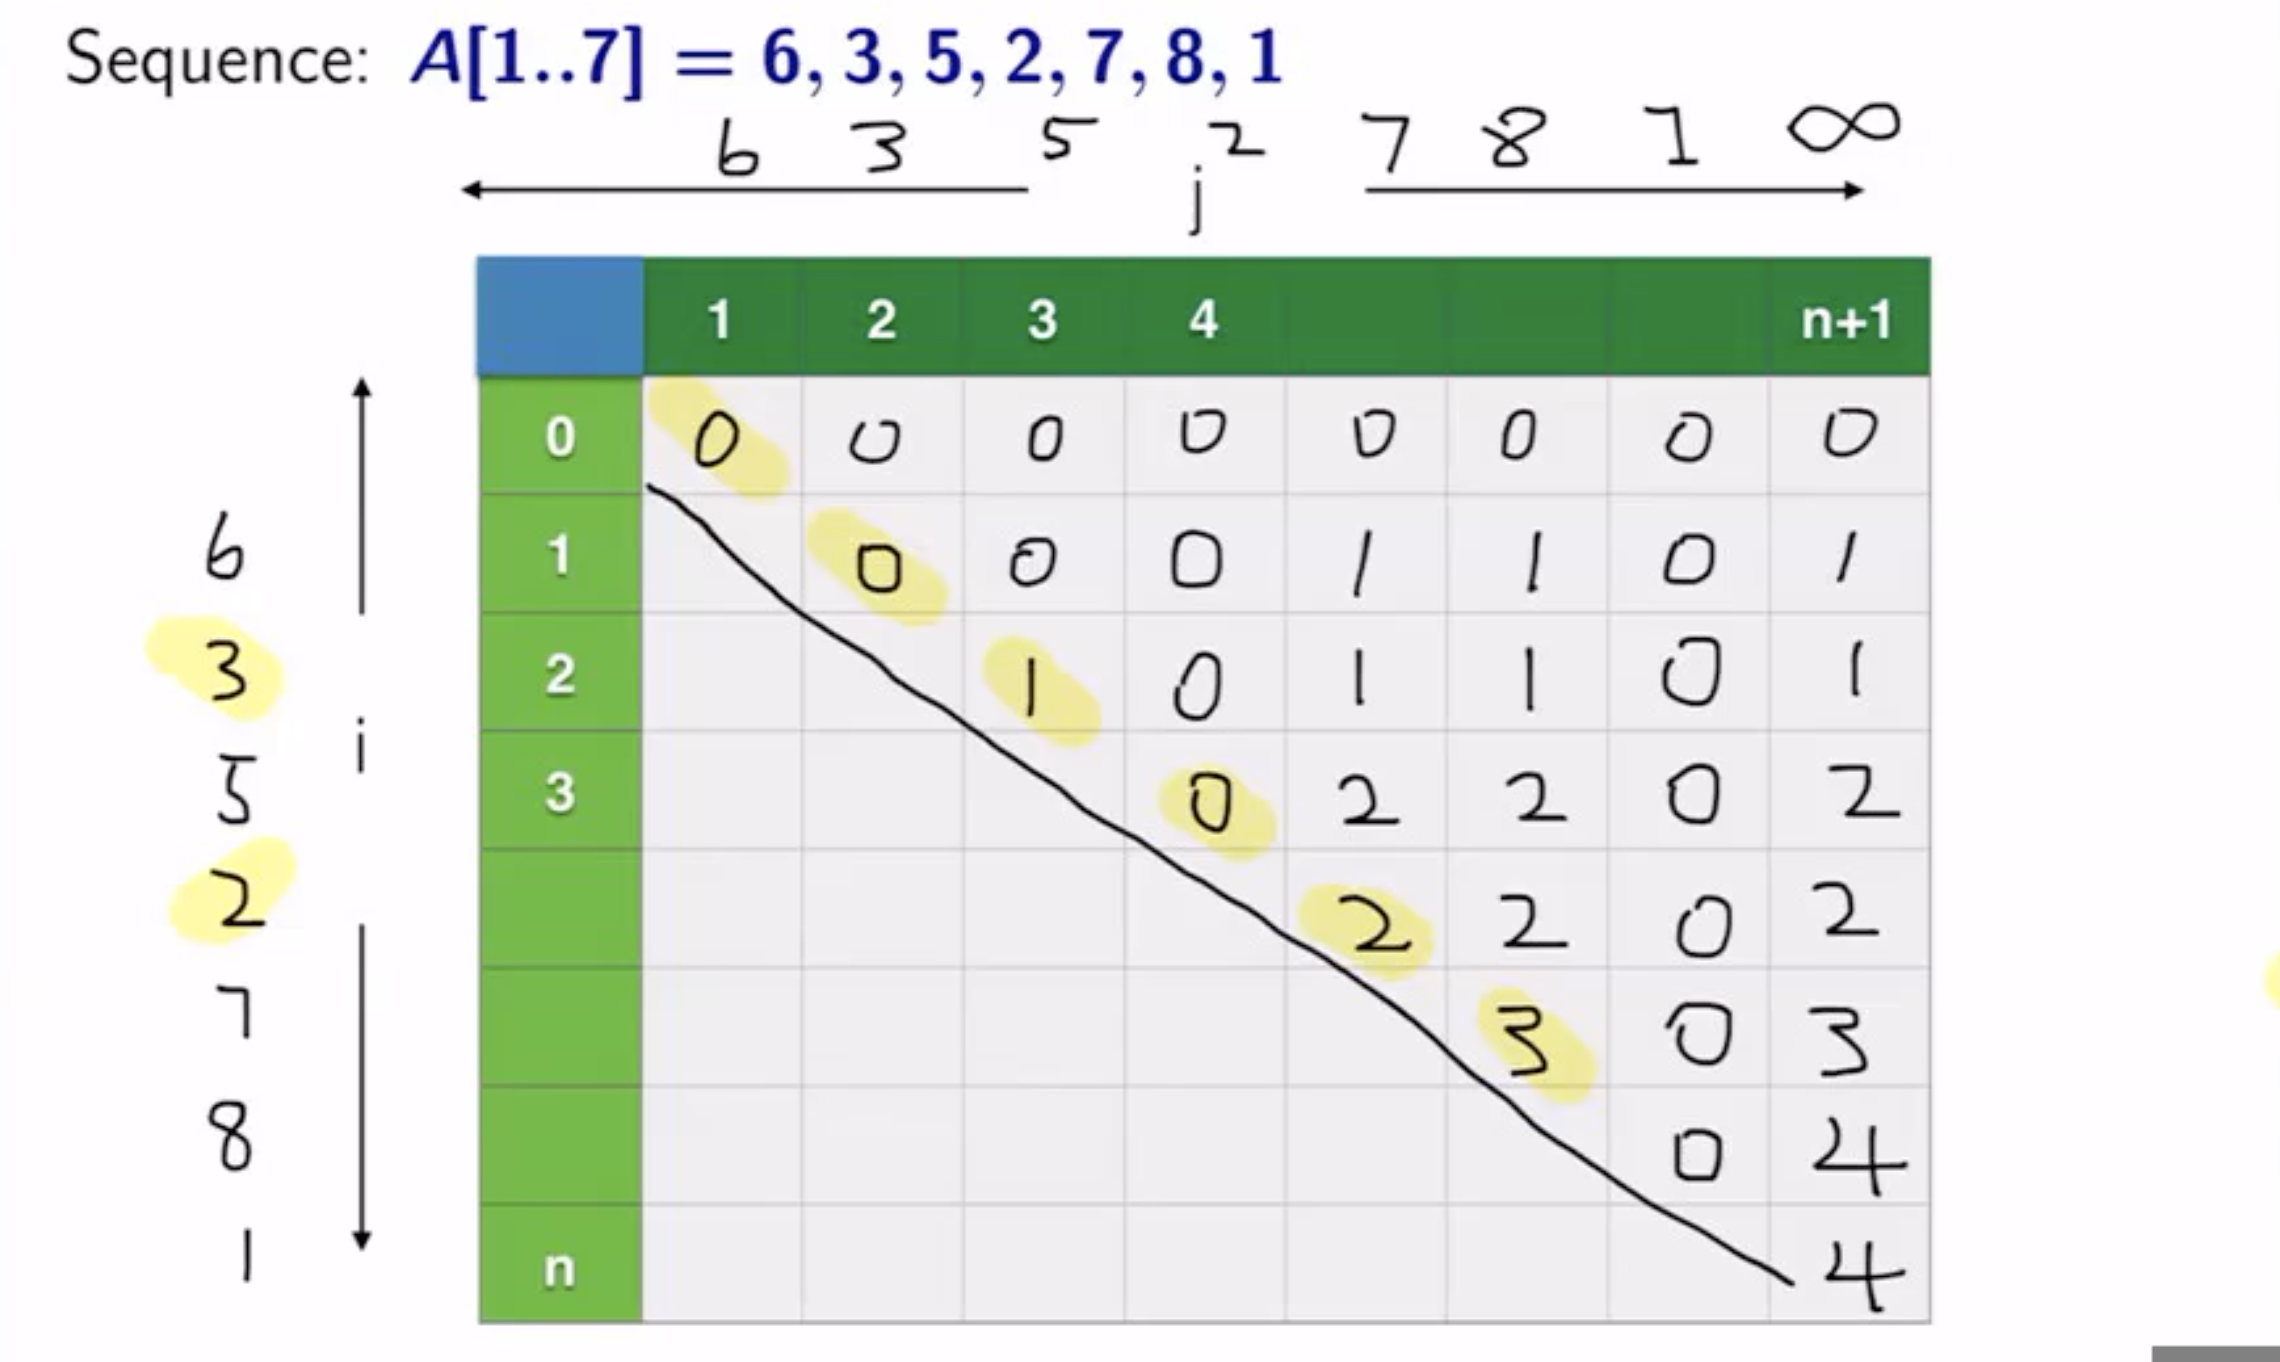
\includegraphics[width=\textwidth]{lecture13/images/lis-memo.png}
\end{itemize}
